\section{Дослідження розроблених алгоритмів}

\subsection{Дослідження розроблених моделі похибок БІНС}

Перевіримо модель та впливи різних складових похимок, на модель БІНС, зобразимо їх в
залежності від часу. Моделювання проведемо над стаціонарно закріпленою БІНС, де
можна перевірити вплив різних джерел помилок.

Для початку перевіримо випадок коли координатний трьохгранник має невеликий нахил,
помилку $\Delta \alpha_{E}$. Це призведе до того, що на горизонтальний акселерометр
подіє прискорення $-g \alpha_{E}$. Виміряне прискорення спричинить, до того, що після
двох інтеграторів, буде здаватись, що система має швидкість і відповідно рухається.
Це спричинить момент на гіроскопах в напрямку зменшення зміщення помилки
координатного трьох гранника, але коли акселерометр стає зрівноваженим система 
матиме значну швидкість, що продовжить коливання. Це нагадує маятник, коли відхиляють
підвіс і дають йому коливатись

На рис. \ref{fig:ins_stat_tilt} зображено результат моделювання руху похибки ІНС
яка зумовлена початковим зміщенням координатного тригранника на $10^{-3} rad$.
Можна зазначити, що помилка коливається з частотою Шулера, з періодом 84.4 хвилини.
Найбільша помилка приблизно 1300 метрів і досягається приблизно за 42.2 хвилини
роботи системи.
\begin{figure}[here]
\centering
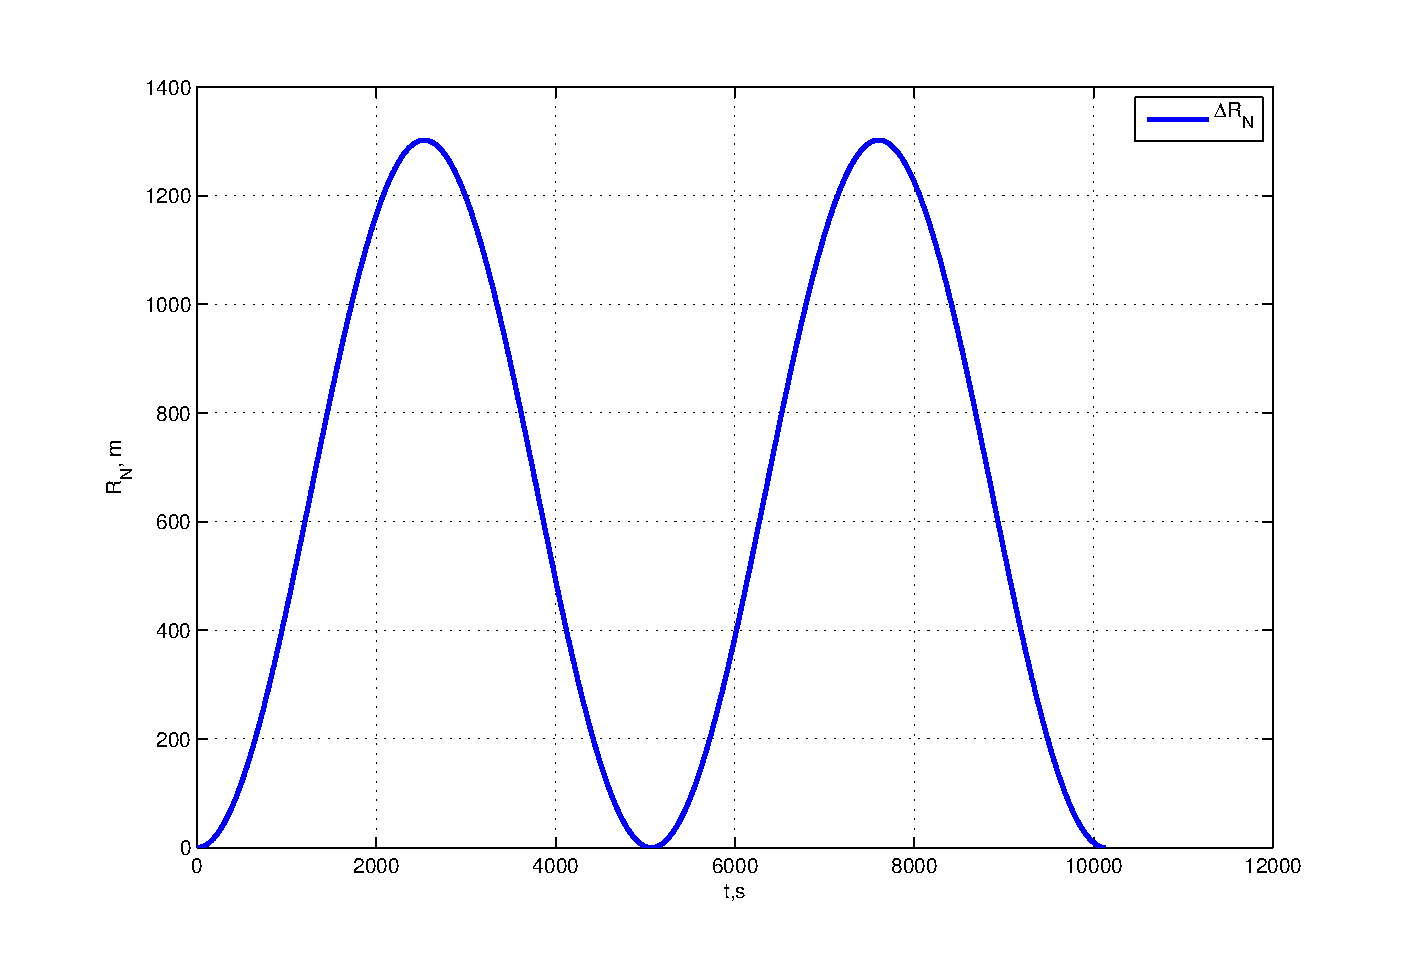
\includegraphics[scale=0.6]{ins_stat_tilt}
\caption{Еволюція похибки за умови, похибки координатного тригранника $10^{-3} rad$}
\label{fig:ins_stat_tilt}
\end{figure}
Розглянемо еволюцію похибок при наявності дрейфа гіроскопа. Ефект дрейфа гіроскопа
позначається на нахилі координатного тригранника, в результаті помилка прискорення.
Швидкість і координата коливаються з частотою Шулера. Але цього разу швидкість
коливається не навколо нуля, отже помилка координати утворюється як сума лінійної
наростаючої та гармонічної функції.

На рис.\ref{fig:ins_stat_gyro} загальна помилка моделюється для стаціонарно
закріпленої ІНС з дрейфом вертикального гіроскопа на $0.01^{o}/h$, яскраво
виражені коливання Шулера та лінійно наростаюча функція. Після 1 години роботи
похибка по координаті приблизно 1300 метрів. Якщо гіроскоп менш точний то його
дрейф спричиняє похибку 1600 метрів за 10 хвилин. Зрозуміло, що на дешевих 
ДПІ похибка зростає до 1500 метрів за 1 хвилину, мала точність 
\begin{figure}[here]
\centering
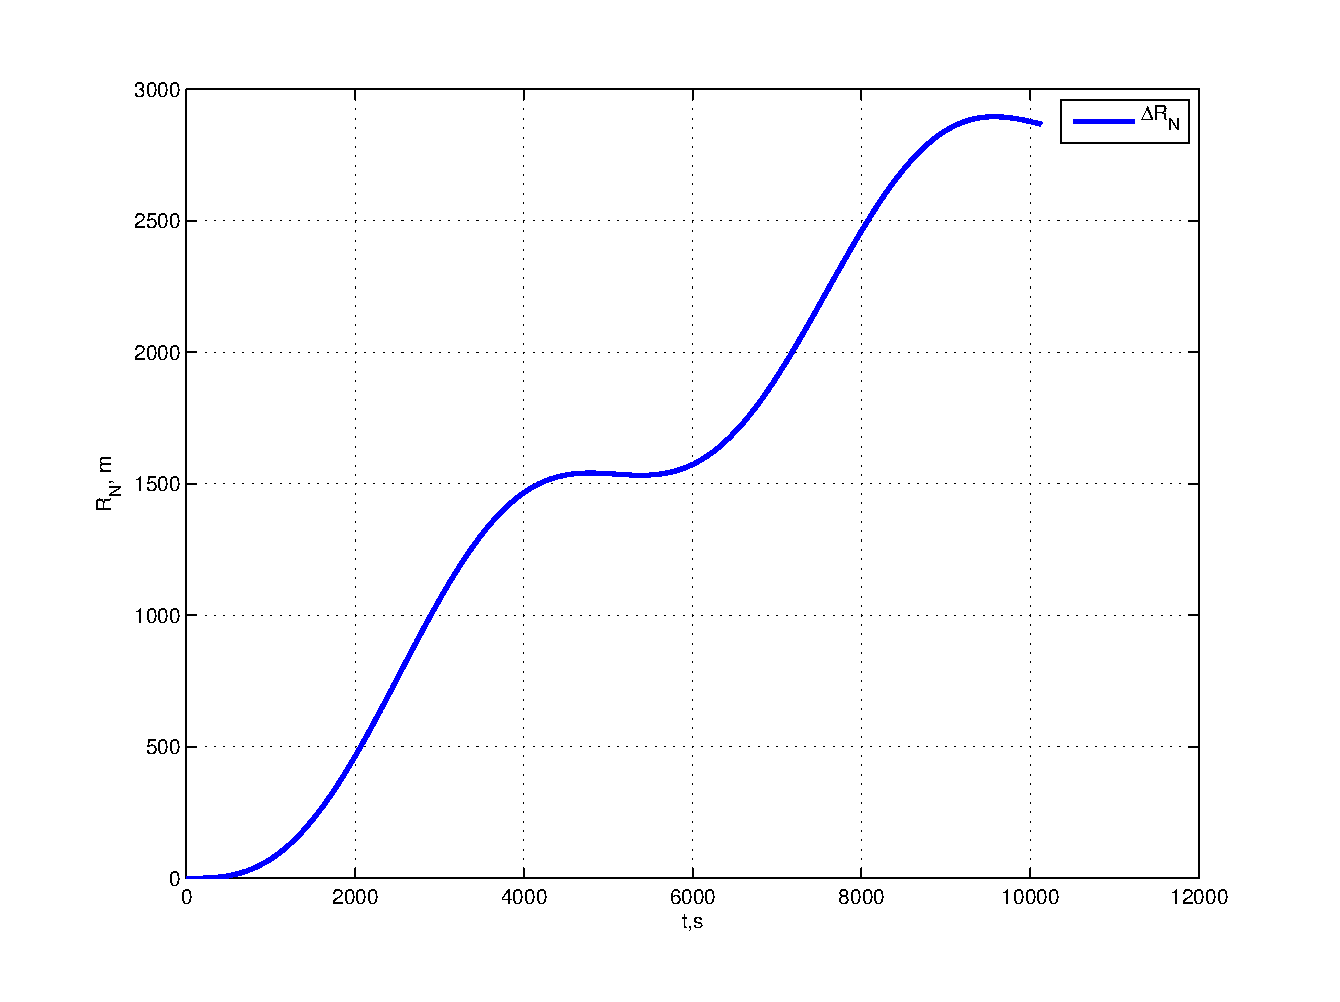
\includegraphics[scale=0.6]{ins_stat_gyro}
\caption{Еволюція похибки за умови, дрейфу гіроскопа $0.01 deg/h$}
\label{fig:ins_stat_gyro}
\end{figure}